\newpage
\section{Auswertung}

Die Abmessungen des Drahtes und die Kugelmasse $m_k$, sowie der Kugelradius $R_k$ ergeben:
\\
\begin{table} [H]
	\centering
	\caption{Abmessungen Draht und Kugel.}
	\label{tab:abmessungen}
	\sisetup{table-format=3.2}
	\begin{tabular}{S[table-format=3.2] S S S S [table-format=3.2]}
		\toprule
		{$\qquad$} & {$l_\text{Draht} / cm$} & {$d_\text{Draht} / mm$} & {$m_k / g$} & {$2R_k / mm$} \\
		\midrule
		&67.00 & 0.16 & 588.3 & 51.03 \\
		&66.00 & 0.17 &\,&\, \\
		&66.00 & 0.16 & \,&\, \\
		&66.00 & 0.16 & \,& \,\\
		&67.00 & 0.17 &\, &\, \\
		&67.00 &\, &\, &\, \\
		&67.00 &\, &\, &\, \\
		&66.00 &\, &\, &\, \\
		&68.00 &\, &\, &\, \\
		&67.00 &\, &\, &\, \\
		\bottomrule 
		{Mittelwert, Gl.(17)} & 66.66 & 0.164 & 588.3 & 51.03 \\
		{Abweichung, Gl.(18)} & 0.0024 & $\num{2.45e-6}$ & $\num{2.4e-4}$ & $\num{2.04e-5}$ 
	\end{tabular}
\end{table}

Der Mittelwert wurde hierbei anhand der Formel 

\begin{equation}
	\overline{x} = \frac{1}{n} \sum_{i=1}^n x_i
\end{equation}

bestimmt. Die Abweichung $\sigma$ mit $i = 1,...,n$:

\begin{equation}
	\sigma_i = \frac{s_i}{\sqrt{n}} = \sqrt{\frac{\sum_{j=1}^n (v_j - \overline{v_i})^2}{n*(n-1)}}
\end{equation}
\newpage

\subsection{Messung ohne B-Feld}
\subsubsection{Schubmodul G}

Für die Schwingungsdauern ergaben sich folgende Werte:

\begin{table} [H]
	\centering
	\caption{Periodendauer der Schwingungen der Kugel ohne magnetisches Feld.}
	\label{tab:T2}
	\sisetup{table-format=3.3}
	\begin{tabular}{S[table-format=3.5] S S [table-format=3.5]}
		\toprule
		{$\qquad$} & {$T / s$} \\
		\midrule
		&18.544\\
		&18.540\\
		&18.551\\
		&18.570\\
		&18.252\\
		&18.537\\
		&18.579\\
		&18.563\\
		&18.554\\
		&18.589\\
		\bottomrule 
		{Mittelwert, Gl.(17)} & 18.528\\
		{Abweichung, Gl(18)} & 0.031\\
	\end{tabular}
\end{table}

Das Schubmodul $G$ wird nun nach Gl.(11) mit den obigen Werten berechnet.
Mit der Fehlerfortpflanzung: 

\begin{equation}
	\increment x_i = \sqrt{(\frac{\partial f}{\partial k_1} * \sigma_{k_1})^2 + (\frac{\partial f}{\partial k_2} * \sigma k_{k_2})^2 + ...}
\end{equation}

\begin{quote}
		$\increment G = \sqrt{(\frac{\partial G}{\partial m_k} * \sigma_{m_k})^2 + (\frac{\partial G}{\partial R_k} * \sigma_{R_k})^2 + (\frac{\partial G}{\partial T} * \sigma_T)^2 + (\frac{\partial G}{\partial d} * \sigma_d)^2 + (\frac{\partial G}{\partial l} * \sigma_l)^2}$
\end{quote}

Somit ist: 
\begin{quote} 
G = $\SI{1.678\pm0.101}{\num{e11}\newton\per\square\metre}$
\end{quote}

\subsubsection{Querkontraktionszahl}

Aus (4)  ergibt sich mit einem Fehler nach (19) 

\begin{quote}
	$\increment \mu = \sqrt{(\frac{\partial \mu}{\partial E} * \sigma_{E})^2 + (\frac{\partial \mu}{\partial G} * \sigma_{G})^2}$
\end{quote}

für die Querkontraktionszahl 

\begin{quote}
	$\mu = -0,37 \pm 0,04$
\end{quote}

Das E-Modul wurde aufgrund der entfallenden Messung wie folgt angegeben: 
\begin{quote}
	E = $\SI{21.00\pm0.05}{\num{e10}\newton\per\square\metre}$
\end{quote}
\subsubsection{Kompressionsmodul}

Aus (5) ergibt sich mit dem Fehler nach (19)

\begin{quote}
	$\increment Q = \sqrt{(\frac{\partial Q}{\partial E} * \sigma_{E})^2 + (\frac{\partial Q}{\partial \mu} * \sigma_{\mu})^2}$
\end{quote}

für das Kompressionsmodul 

\begin{quote}
	$Q = \SI{4.00\pm0.17}{\num{e10}\pascal}$
\end{quote}


\subsection{Messung mit B-Feld}

Für die Schwingungsdauern im Abhängigkeit von der Stromstärke, bzw. dem Magnetfeld, ergaben sich folgende Werte:
\begin{table} [H]
	\centering
	\caption{Periodendauer der Schwingungen der Kugel mit magnetischem Feld (0.5A-2-5A).}
	\label{tab:T3.1}
	\sisetup{table-format=1.3}
	\begin{tabular}{S[table-format=1.5] S S S S S S}
		\toprule
		& & \multicolumn{3}{c}{$T / s$} \\
		\cmidrule(lr){4-4}
		{$I$ / A} && {0.5\;} & {1.0\;} & {1.5 \;} & {2.0 \;} & {2.5} \\
		\midrule
		&&11.310&8.756&7.467&6.583&5.975\\
		&&11.102&8.779&7.465&6.608&5.973\\
		&&11.101&8.762&7.460&6.596&5.981\\
		\bottomrule
		{Mittelwert, Gl.(17)}&& 11.17 & 8.766& 7.464& 6.596& 5.976\\
		{\, Abweichung, Gl(18)}&& 0.07 & 0.007& 0.002& 0.007& 0.0024\\
	\end{tabular}
\end{table}

\begin{table} [H]
	\centering
	\caption{Periodendauer der Schwingungen der Kugel mit magnetischem Feld(3.0A-5.0A).}
	\label{tab:T3.2}
	\sisetup{table-format=1.3}
	\begin{tabular}{S[table-format=1.5] S S S S S S}
		\toprule
		& & \multicolumn{3}{c}{$T / s$} \\
		\cmidrule(lr){4-4}
		{$I$ / A} && {3.0 \;} & {3.5 \;} & {4.0 \;} & {4.5 \;} & {5.0} \\
		\midrule
		&&5.521&5.136&4.538&4.558&4.336\\
		&&5.526&5.132&4.577&4.587&4.330\\
		&&5.519&5.142&4.865&4.556&4.344\\
		\bottomrule
		{Mittelwert, Gl.(17)}&& 5.522& 5.137& 4.67& 4.567&4.337 \\
		{\, Abweichung, Gl(18)}&& 0.002& 0.003& 0.1& 0.01&0.004\\
	\end{tabular}
\end{table}
\newpage

Nach Gleichung (15) mit $N = 80$ und $R_\text{H} = \SI{72}{\milli\metre}$ können die $B$-Werte im folgenden $\frac{1}{T^2} - B$ Diagramm wiedergegeben werden:

\begin{figure}[h]
  \centering
  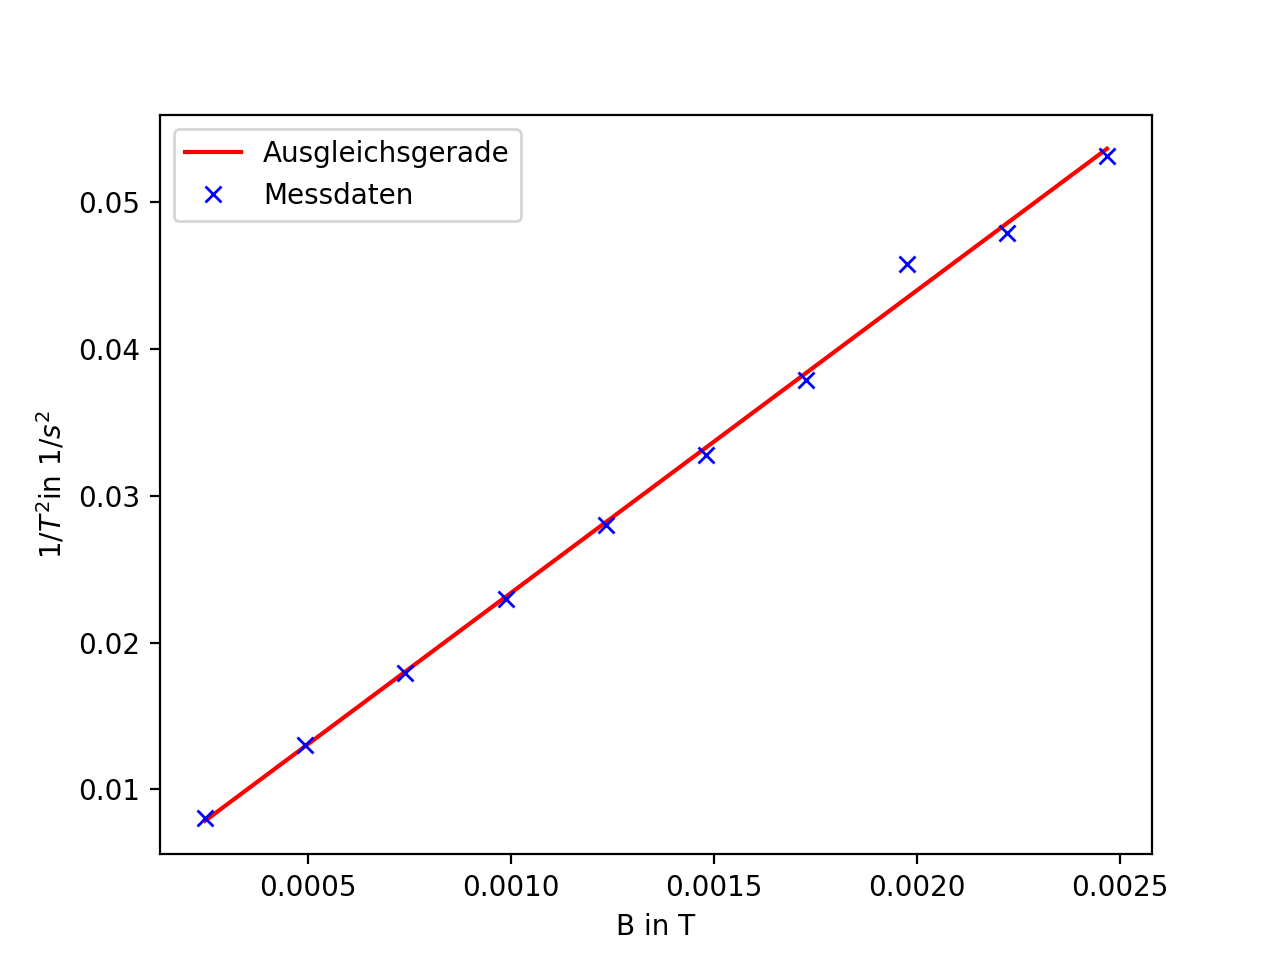
\includegraphics[height=10cm]{Auswertung/Graph.png}
  \caption{1/T - B Diagramm zur Berechnung des magn. Momentes.}
  \label{fig:Graph}
\end{figure}

Über Formel
\begin{equation}
	m\cdot x + b
\end{equation}
wird die Steigung und der Fehler der Ausgleichsgerade von Python Modul Scipy Curve fit berechnet.

\begin{gather}
	a = 10.187 \pm 0.040 =: \frac{1}{T^2*B} \notag \\
	b = 0.0027 \pm \num{3.82e-7}	\notag
\end{gather}

Die Ausgleichsgerade hat somit die Form:

\begin{quote}
	$(10.187 \pm 0.040)*x + (0,0027 \pm \num{3,82e-7})$
\end{quote}

Mit Gleichung (10), (16) und (19) ergibt sich für das magnetische Moment $m_{magn}$ die Formel:

\begin{equation}
	m_{magn} = \frac{4 \pi^2}{B*T^2}*\theta - \frac{D}{B} = 4 \pi^2*m*\theta - \frac{D}{B}
\end{equation}
\newpage

Nach (16) und (19) ergibt sich dann mit der Fehlerfortpflanzung

\begin{quote}
	$\increment m_\text{magn} = \\
	\\
	\sqrt{(\frac{\partial m_{magn}}{\partial m} * \sigma_{m})^2 + (\frac{\partial m_{magn}}{\partial R_k} * \sigma_{R_k})^2+(\frac{\partial m_{magn}}{\partial M_k} * \sigma_{M_k})^2+(\frac{\partial m_{magn}}{\partial D} * \sigma_{D})^2(\frac{\partial m_{magn}}{\partial \overline{B}} * \sigma_{\overline{B}})^2}$
\end{quote}

das magnetische Moment

\begin{quote}
	$m_\text{magn} = \SI{0.05601\pm0.00028}{\ampere\square\metre}$
\end{quote}






